% -*- mode: fundamental -*-

% ****************************************************************

\chapter{RISC-V: Core functions for RISC-V ISA execution (used in Drum and Fife)}

\markboth{Ch \arabic{chapter}: RISC-V: Core functions}{\copyrightnotice}

\setcounter{page}{1}
% \renewcommand{\thepage}{\arabic{page}}
\renewcommand{\thepage}{\arabic{chapter}-\arabic{page}}

\label{ch_core_functions}

% ****************************************************************

\section{Introduction}

In this chapter we discuss the core functions of
Figure~\ref{Fig_Core_Simple_Instr_Exec}: \verb|fn_Fetch|,
\verb|fn_Decode|, \verb|fn_Dispatch|, \verb|fn_EX_Control| and
\verb|fn_EX_Int|.
\begin{figure}[htbp]
  \centerline{\includegraphics[width=6in,angle=0]{Figures/Fig_Instr_Exec_w_structs}}
  \caption{\label{Fig_Core_Simple_Instr_Exec}
           Simple interpretation of RISC-V instructions}
\end{figure}

% ****************************************************************

\section{The function {\tt fn\_Fetch}}

\label{Sec_fn_Fetch}

\index[RV]{fn\_Fetch@{\tt fn\_Fetch} (Fetch function)}
\index[RV]{Fetch function ({\tt fn\_Fetch})}

The Fetch function \emph{per se} is fairly simple, even trivial.  Its
input is the current value of the program counter (PC), which is used
as the address in a memory-request to IMem.  It has two outputs,

\begin{tightlist}

 \item A \emph{memory request} to memory, to read an instruction.  We
       have already seen the definitition of the \verb|Mem_Req| struct
       in Section~\ref{Sec_Mem_Req}.

 \item Some additional information ``\verb|Fetch_to_Decode|'' passed
       on to the Decode step.

\end{tightlist}

The ``\verb|Fetch_to_Decode|'' struct has only one interesting field,
the PC:

\input{Code_Extracts/Fetch_to_Decode.tex}

The field \verb|inum| holds the ``instruction number'', which is a
sequence number counting every instruction fetched.  It is used only
for debugging, to be able to identify a specific fetched instruction.
(In the source code you will see two more fields \verb|predicted_pc|
and \verb|epoch|; ignore these for now, they are not used in Drum,
only in Fife.)

\index[BSV]{struct!nested}

To pass both results of \verb|fn_Fetch|, we simply use a \emph{nested}
struct, {\ie} a struct containing the two component structs:

\input{Code_Extracts/Result_F.tex}

Finally, as mentioned earlier, the function \verb|fn_Fetch| is almost
trivial: it merely fills in the two result structs based on argument
values and returns them:

\input{Code_Extracts/fn_Fetch.tex}

As the comment at the top of the code excerpt says, \verb|fn_Fetch| is
actually a pure function (no side-effects), and we could have written
it as follows:

{\small
\begin{Verbatim}[frame=single, numbers=left]
function Result_F
         fn_Fetch (Bit #(XLEN)  pc,
		   ...
		   Bit #(64)    inum);
      Result_F y = ?;
      ...
      return y;
endfunction
\end{Verbatim}
}

{\ie} the return-type is \verb|Result_F| instead of
\verb|ActionValue#(Result_F)|, and we simply drop the
``\verb|actionvalue|---\verb|endactionvalue|'' bracket
keywords. Recall Section~\ref{Sec_Pure_vs_Side_Effect_functions} where
we discussed pure {\vs} side-effecting functions, and their
distinction in the type-system through the absence/presence of the
\verb|ActionValue| type constructor.  Even though this is a pure
function, by couching it as an \verb|ActionValue| type, we preserve
the option of inserting a \verb|$display| (which \emph{is} a
side-effect) for debugging purposes, should we need it in the future.

In line 9 we declare variable \verb|y| of type \verb|Result_F|, with
unspecified initial value (recall Section~\ref{Sec_Dont_Care_Values}
where we discussed using ``\verb|?|'' to indicate an unspecified or
don't-care value).  The two fields of \verb|y| are then updated in
lines 11 and 14, respectively, and \verb|y| is finally returned as the
result of the function.

We also use ``\verb|?|'' in line 17 the \verb|data| field is only
relevant in a STORE memory request, whereas this is a FETCH request.

% ================================================================

\hdivider

% ----------------
\Exercise

Write a testbench for \verb|fn_Fetch()|, apply it to a number of
32-bit values (PC values) and print the results using \verb|$display|
and \verb|fshow|, and visually check that the \verb|Fetch_to_Decode|
and \verb|Mem_Req| outputs look correct.

\Endexercise

% ****************************************************************

\section{The {\tt fn\_Decode} function}

\label{Sec_fn_Decode}

\index[RV]{fn\_Decode@{\tt fn\_Decode} (Decode function)}
\index[RV]{Decode function ({\tt fn\_Decode})}

The core function for the Decode step is called \verb|fn_Decode|.  Its
arguments are a struct of type \verb|Fetch_to_Decode| from the Fetch
step and a \verb|Mem_Rsp| memory response struct from memory.  Its
output struct type, \verb|Decode_to_RR|, was described in
Section~\ref{Sec_struct_D_to_RR}.  The code for \verb|fn_Decode| is
mostly a big if-then-else that analyses the incoming instruction and
produces some summary information:

\input{Code_Extracts/fn_Decode.tex}

\index[BSV]{truncate@{\tt truncate}, operation to shrink bit-width}

In line 6, we extract the instruction from the \verb|Mem_Rsp| memory
response \verb|data| from the Fetch operation. The \verb|truncate|
operation is used to shrink the bit-vector width of
\verb|rsp_IMem.data| (64 bits) to the bit-vector width of \verb|instr|
(32 bits).  (Section~\ref{Sec_Mem_Req} discussed why we declared
\verb|rsp_IMem.data| to be 64-bits wide).  The \verb|truncate|
operation is polymorphic, accepting arguments of any bit-width that is
at least as wide as the required output.  Note, \verb|truncate| keeps
least-significant bits and drops most-significant bits.

In line 7 we extract the \verb|rd| (``destination register'') field
from the instruction.  In line 9 we compute the fall-through PC, PC+4
(with the caveat that if extend the implementation to support the
``C'' RISC-V ISA extension (``Compressed'' instructions), it may be
PC+2, which information can be gleaned from the instruction encoding).

In lines 11-26 we create a baseline \verb|Decode_to_RR| value which we
will selectively modify in the if-then-else statements that follow.

In lines 31-40 we first handle the sitations where the Fetch operation
to memory itself returned an error.  We mark the \verb|exception|
field True and fill in the appropriate \verb|cause| and \verb|tval|
(these will be placed in MCAUSE and MTVAL CSRs in the Retire step).

The rest of the code is a series of if-then-else clauses. Each clause
identifies one class of instruction and updates the \verb|opclass|
field correspondingly.  The repertoire of instructions that we
consider are the forty instructions listed in the ``RV32I Base
Instruction Set'' table of ``Table 24.2: Instruction listing for
RISC-V'' of the Unprivileged Spec~\cite{RISCV_Unpriv_2019_12_13}.

Each if-then-else clause also fills in the \verb|has_rs1|,
\verb|has_rs2| and \verb|has_rd| fields, as appropriate, for each
class of instruction.  Note that the \verb|has_rd| field is set to
False if \verb|rd| is zero (recall that general-purpose register
\verb|x0| ignores writes and always reads as 0).

We also decode each kind of ``immediate'' and fill in the \verb|imm|
field in the struct.  Recall from
Section~\ref{Sec_Instruction_Encodings}, including
Figures~\ref{Fig_J_imm} and \ref{Fig_B_imm}, that different classes of
instructions encode immediate values in different ways, and the
immediate values can have different bit-widths.  We use the functions
\verb|instr_imm_I()|, \verb|instr_imm_S()|, \verb|instr_imm_B()|,
\verb|instr_imm_U()| and \verb|instr_imm_J()| to extract the and
rearrange the immediate bits appropriately for each class of
instruction.  Then, here in \verb|fn_Decode|, we zero- or sign-extend
each immediate as appropriate so that, from this point onwards, each
immediate can be treated as an ordinary \verb|Bit#(XLEN)| value.

An exercise below suggests that you write the code for these
\verb|instr_imm_X| functions; it's good practice for the BSV beginner!

The final ``else'' clause is selected if the instruction does not
match any of the forty RV32I instructions.  In this case we set the
\verb|exception| field, and set the \verb|cause| field to indicate an
illegal instruction.

Observe that the entire \verb|fn_Decode()| function is just a (large)
combinational circuit---it is an acyclic composition of smaller
combinational circuits, many of which we've seen earlier.  The whole
\verb|fn_Decode()| function can be visualized as a box with incoming
wires corresponding to the \verb|Fetch_to_Decode| struct and the
\verb|Mem_Rsp| struct, outgoing wires corresponding to the
\verb|Decode_to_RR| struct, and filled with logic gates that compute
each output wire as a function of the input wires.

% ================================================================

\hdivider

% ----------------
\Exercise

The provided source code includes the functions \verb|instr_imm_I()|,
\verb|instr_imm_S()|, \verb|instr_imm_B()|, \verb|instr_imm_U()| and
\verb|instr_imm_J()| (in file \verb|Instr_Bits.bsv|), but try to write
them yourself first, and compare your solutions to the provided codes.

% ----------------
\Exercise

Write a testbench for \verb|fn_Decode()|, apply it to a number of PC
and instruction values.  For each input PC value, construct an
\verb|Fetch_to_Decode| struct around it.  For each input instruction,
construct a \verb|Mem_Rsp| struct around it, some with memory errors,
some without.  Apply \verb|fn_Decode| to such pairs.  Print the
results results using \verb|$display| and \verb|fshow|, and visually
check that the \verb|D_to_RR| outputs look correct.

\Endexercise

% ****************************************************************

\section{The {\tt fn\_Dispatch} function after reading input registers}

\label{Sec_fn_Dispatch}

\index[RV]{fn\_Dispatch@{\tt fn\_Dispatch} (Dispatch function)}
\index[RV]{Dispatch function ({\tt fn\_Dispatch})}

In the Register-Read and Dispatch step (``RR'', ``RRD''), we first
read the \verb|rs1| and \verb|rs2| values from the Register File.  We
will cover register files in Section~\ref{Sec_Register_files}, and
register-reads when we discuss the Drum CPU itself, in
Chapter~\ref{ch_Drum_code}.

With the \verb|rs1| and \verb|rs2| values in hand, we use function
\verb|fn_Dispatch| to determine the information to be passed to the
various alternative steps (``flows'') that follow.  Its argument is a
\verb|Decode_to_RR| struct from the Decode step, which was discussed
in Section~\ref{Sec_struct_D_to_RR}.  Before we look at the result
type of \verb|fn_Dispatch|, let us discuss the four possible
subsequent flows:

\begin{itemize}

  \item ``Direct'': Some information is sent directly from RR to
        Retire for \emph{every} instruction.  Crucially, RR sends a
        \emph{tag} that indicates which of the four flows is being
        followed for the current instruction.

        Additional direct information includes information from RR
        (PC, whether an exception has already been seen in the Fetch
        or Decode stages, \verb|has_rd|, \verb|writes_mem|, the
        instruction, the fall-through PC and the \verb|rs1| value
        (needed for CSRRx instructions).

       The direct flow is also used for all SYSTEM instructions,
       including CSRRxx, ECALL, EBREAK, and MRET.

  \item ``Control'': If the instruction is a BRANCH, JAL or JALR, we
        produce information for the Execute Control flow.

  \item ``Integer'': If the instruction is a LUI, AUIPC or integer
        arithmetic or logic (IALU) operation, we produce information
        for the Execute Integer flow.

  \item ``DMem'': If the instruction is a LOAD, STORE or FENCE, we
        produce information for the Execute Memory flow.

\end{itemize}

The following enum type declaration defines four constants to identify
the flow for this instruction:

\input{Code_Extracts/Exec_Tag.tex}

The result type of \verb|fn_Dispatch| is \verb|Result_Dispatch|.  It
is just a nested struct that contains four different struct types for
the four flows (the struct types can be seen on arc labels in
Figure~\ref{Fig_Core_Simple_Instr_Exec}).

\input{Code_Extracts/Result_Dispatch.tex}

The first component is the information sent directly to Retire:

\input{Code_Extracts/RR_to_Retire.tex}

The \verb|exec_tag| informs Retire about the flow for this
instruction.  The {\tt exception} and {\tt cause} fields from
\verb|Decode_to_RR| are carried through, as-is, since it is the Retire
step that handles all exceptions.  Note, in addition to passing these
exceptions in RR to Retire, the Control or Execute steps can also
produce exceptions.  The {\tt pc} field is needed in case Retire needs
to handle a trap or interrupt, which saves the {\tt pc} before
handling it.

The \verb|has_rd| field is carried through to control whether Retire
tries to write a value back to the register file nor not.  The
\verb|fallthru_pc| is used for most instructions that complete
successfully (without raising an exception).

The second component of \verb|Result_Dispatch| is the information sent
to Execute Control (we will see how these fields are used in
Section~\ref{Sec_fn_EX_Control} when we discuss \verb|fn_EX_Control|):

\input{Code_Extracts/RR_to_EX_Control.tex}

The third component of \verb|Result_Dispatch| is the information sent
to Execute Int (we will see how these fields are used in
Section~\ref{Sec_fn_EX_Int} when we discuss \verb|fn_EX_Int|):

\input{Code_Extracts/RR_to_EX.tex}

We choose to call it \verb|RR_to_EX| instead of \verb|RR_to_EX_Int|
because the same struct type is likely to be used in future also for
the other optional execution pipes shown in
Figure~\ref{Fig_Core_Simple_Instr_Exec}: Integer Multiply Divide
(``M'' ISA extension), floating point (``F'' and ``D'' ISA extensions)
and Custom (non-standard ISA extensions).

The third component of \verb|Result_Dispatch| is the information sent
to Execute DMem, and is the same \verb|Mem_Req| struct we have already
discussed in Section~\ref{Sec_Mem_Req}, and which is also an output
component of \verb|fn_Fetch|.

The code for \verb|fn_Dispatch| is shown below.  Its arguments are the
\verb|Decode_to_RR| struct from the Decode stage, and values from the
source registers \verb|rs1| and \verb|rs2|.

\input{Code_Extracts/fn_Dispatch.tex}

Lines 7-14 compute \verb|exec_tag|, {\ie} the flow to be followed.

Lines 16-29, 33-38, 42-46 and 49-61 construct the flow-specific struct
values.  The latter three are meaningful only if \verb|exec_tag|
indicates Control, Integer of DMem, respectively, but there is no harm
in constructing them, even if they may contain bogus data; they will
only be used when their flows are chosen and ignored otherwise.

Lines 64-68 construct and return the final result with the four
component structs.

% ****************************************************************

\section{The {\tt fn\_EX\_Control} function}

\label{Sec_fn_EX_Control}

\index[RV]{fn\_EX\_Control@{\tt fn\_EX\_Control} (Execute Control function)}
\index[RV]{Execute Control function ({\tt fn\_EX\_Control})}

This function is a simple one-input one-output function.  The input
type \verb|RR_to_EX_Control| was described in
Section~\ref{Sec_fn_Dispatch}, where it was an output type.  The
output type of \verb|fn_EX_Control| is shown below:

\input{Code_Extracts/EX_Control_to_Retire.tex}

Here is the Execute Control function:

\input{Code_Extracts/fn_EX_Control.tex}

The first ``\verb|if|'' clause handles BRANCH (conditional branch)
instructions.  The \verb|case| expression computes the boolean value
\verb|branch_taken|, {\ie} the decision whether to take the branch or
not.  A case-clause is chosen based on the 3-bit \verb|funct3| field
of the instruction that identifies the specific condition to be
tested.\footnote{Unlike C/C++, where a case-clause ``falls through''
to the next case-clause unless you have a {\tt break} statement, in
BSV only one case-clause is executed, there is no fall-through.}  Note
that for BLT and BGE, we use BSV library functions \verb|signedLT| and
\verb|signedGE| that interpret \verb|rs1_val| and \verb|rs2_val| as
2's-complement signed integers.

Line 16 computes the target PC should the the branch be taken.  Line
17 computes the next PC, which is either the target PC or the
fall-through PC depending on whether or not the branch is taken.
Finally, Line 18 checks, if the branch is taken, that the target PC is
a properly aligned address (if not, we must raise an exception).

The next ``\verb|else if|'' clause handles JAL (Jump and Link)
instructions and the final ``\verb|else if|'' clause handles the JALR
(Jump and Link Register) instructions.  They are both straightforward,
unconditional calculations of a next PC, along with an alignment-check
that the next PC is suitably aligned.  As per the Unprivileged ISA
specification document, JALR also zeroes the least-significant bit of
target PC.

The final section constructs the \verb|EX_Control_to_Retire| struct
result and returns it.

\vspace*{2ex}

\hdivider

% ----------------
\Exercise

In {\tt fn\_EX\_Control}, the BRANCH, JAL and JALR clauses set the
{\tt exception} field to true if the next PC is not aligned.

\begin{enumerate}

  \item What would happen if we did not set the exception field here?

  \item See ``Section 2.5 Control Transfer Instructions'' in the
      Unprivileged ISA specification document
      \cite{RISCV_Unpriv_2019_12_13}) for a discussion of why we set
      it here.

\end{enumerate}

% ----------------
\Exercise

Prove (informally) that the three-way if-then-else shown above in
\verb|Fn_EX_Control| will catch all cases, {\ie} that we never need a
final ``\verb|else|'' clause.  This requires reviewing
\verb|fn_Decode| and tracking the flow of information through the
Register-Read-and-Dispatch step (including \verb|fn_Dispatch)|, into
\verb|fn_Control|.

% ----------------
\Exercise

In \verb|Fn_EX_Control|, can we change the final ``\verb|else if|'':

{\small
\begin{Verbatim}[frame=single]
   else if (is_JALR (instr)) begin
\end{Verbatim}
}

into a simple ``\verb|else|'', {\ie} omit the the \verb|is_JALR|
check?

{\small
\begin{Verbatim}[frame=single]
   else begin
\end{Verbatim}
}

What might be the hardware implication of such a change?

% ----------------
\Exercise

In the final section of {\tt fn\_EX\_Control}, why do we have:
\verb|data: x.fallthrough_pc|? \\
\emph{Hint}: review the semantics of JAL and JALR instructions.

What if this is a BRANCH instruction?

What if this is a JAL or JALR instruction with \verb|rd| = 0?

\Endexercise

% ****************************************************************

\section{The {\tt fn\_EX\_Int} function}

\label{Sec_fn_EX_Int}

\index[RV]{fn\_EX\_Int@{\tt fn\_EX\_Int} (Execute Integer function)}
\index[RV]{Execute Integer function ({\tt fn\_EX\_Int})}

This function is a simple one-input one-output function.  The input
type \verb|RR_to_EX| was described in Section~\ref{Sec_fn_Dispatch},
where it was an output type.  The output type of \verb|fn_EX_Int| is
shown below:

\input{Code_Extracts/EX_to_Retire.tex}

We choose to call it \verb|EX_to_Retire| instead of
\verb|EX_Int_to_Retire| because the same struct type is likely to be
used in future also for the other optional execution pipes shown in
Figure~\ref{Fig_Core_Simple_Instr_Exec}: Integer Multiply Divide
(``M'' ISA extension), floating point (``F'' and ``D'' ISA extensions)
and Custom (non-standard ISA extensions).

Here is the Execute Integer function:

\input{Code_Extracts/fn_EX_Int.tex}

The first ``\verb|if|'' handles LUI instructions (Load Upper
Immediate).  The following ``\verb|else if|'' handles AUIPC
instructions (Add Upper Immediate to PC). The final ``\verb|else|''
handles all the remaining Integer ops by invoking an ``ALU'' function:

\input{Code_Extracts/fn_IALU.tex}

The reason we create a separate \verb|fn_IALU| function, instead of
inlining it into \verb|Fn_EX_Int| is because \verb|fn_IALU| is not
very RISC-V specific, and may be useful in other contexts that have
nothing to do with RISC-V, Drum or FIfe.

In lines 11-13, we define signed-integer versions {\tt iv1}, {\tt iv2}
and \verb|i_imm| of the unsigned integer values {\tt v1}, {\tt v2},
and {\tt imm}, respectively, using the standard BSV \verb|unpack|
function.  There is no hardware cost to this, these declarations are
simply declarations to ``view'' the same bits differently (as
2's-complement coded integers).  The difference arises later, when we
apply certain operators to these values.  For example, lines 24-25
compute the SLT (Set Less Than (signed)) and SLTU (Set Less Than
Unsigned) operations.  SLT uses the signed values {\tt iv1} and {\tt
iv2}, whereas SLTU uses the unsigned values {\tt v1} and {\v2}.
Between the \emph{bsc} compiler and the Verilog back-end, different
code will be generated for the ``{\tt <}'' operator to perform the
correct kind of comparison.

Line 18 extracts a 5-bit ``shift amount'' from the {\tt rs2} value for
the shift operators SLL, SRL and SRA.  Line 39 extract a 5-bit ``shift
amount'' from the {\tt imm} value for the shift operators SLLI, SRLI
and SRAI.

SRL (Shift Right Logical) and SRA (Shift Right Arithmetic) differ in
whether they treat the argument as a signed or unsigned value, the
difference being whether the new bits shifted into the
most-significant bit are zero (SRL) or replicate the most-significant
bit (SRA).  SRLI and SRAI exhibit a similar difference.

In lines 28 (SRA) and 49 (SRAI) we finally apply the ``{\tt pack}''
operator to produce the result. This is because the expression
``\verb|(iv1 >> shamt)|'' has type {\tt Int\#(XLEN)} whereas the
result needs to be of type {\tt Bit\#(XLEN)}.  The ``{\tt pack}''
operator performs this type-change for us.

Lines 19-32 define the \verb|y_OP| result when the opcode is
\verb|opcode_OP| {\ie} {\tt 7'b\_011\_0011}, {\ie} the ``3-address''
operators where the inputs come from {\tt rs1} and {\tt rs2}.
\verb|y_OP| defaults to 0 when it is not an {\tt op\_OP}.

Lines 40-49 define the \verb|y_OP_IMM| result when the opcode is {\tt
opcode\_OP\_IMM} {\ie} {\tt 7'b\_001\_0011}, {\ie} the ``2-address''
operators where one input come from {\tt rs1} and the other input
comes from an immediate value in the instruction.  \verb|y_OP_IMM|
defaults to 0 when it is not an \verb|op_OP_IMM|.

Finally, line 45 combines these results using the ``OR'' function.  We
rely on the fact that exactly one of \verb|y_OP| and \verb|y_OP_IMM|
can be relevant; the other one must be zero (and therefore has no
effect through the OR'ing).

\hdivider

% ----------------
\Exercise

Lines 11-45 could instead have been written this way:

{\small
\begin{Verbatim}[frame=single, numbers=left]
   Bit #(XLEN) y = 0;
   if (opcode == opcode_OP) begin
      ...
      ... y = ...
   end
   else if (opcode == opcode_OP_IMM) begin
      ...
      ... y = ...
   end
   return y;
\end{Verbatim}
}

Discuss the hardware tradeoffs between writing it in these two ways.
{\emph Hints:} Consider:

\begin{tightlist}

  \item Sequentiality of if-then-else.
  \item Ability (or not) to prove exhaustiveness of conditions in nested if-then-else.
  \item Ability (or not) to prove mutual-exclusivity of conditions in nested if-then-else.
  \item Discussion in Section~\ref{Sec_MUXes} on parallel and
    sequential multiplexers (mux).  Note: in our code, we have
    explicitly coded a parallel mux.

\end{tightlist}

% ----------------
\Exercise

Note that the ISA has ADD and ADDI instructions, but no corresponding
SUB and SUBI (subtract) instructions.  Why not?

% ----------------
\Exercise

Justify the presence or absence of the ``{\tt pack}'' operator in each
case of {\tt fn\_IALU}.

% ----------------
\Exercise

Suppose we want to extend {\tt fn\_IALU} so it also works when XLEN=64
({\ie} for RV64I).  What needs to change to accommodate this?

\emph{Hint:} it only matters in the shift-amount of the shift
instructions, where the shift-amount can be 6-bits wide instead of
5-bits (allowing a maximum of 63-bit shifts instead of 31 bits).

\Endexercise

% ****************************************************************

\section{No separate functions for Execute DMem and Retire}

We don't need any separate functions for the Execute DMem step in
Figure~\ref{Fig_Core_Simple_Instr_Exec} because \verb|fn_Dispatch| has
created a \verb|Mem_Req| struct that we can send directly to memory.
Similarly, the memory returns a \verb|Mem_Rsp| that is sent directly
to the Retire step.

The code for the Retire step is discussed in detail separatly in
Chapter~\ref{ch_Drum_code} for Drum and Chapter~\ref{ch_Fife_code} for
Fife.  Although functionally the same, the codes are structurally
sufficiently different that it is not worth attempting to abstract any
common functionality into a shared function.

% ****************************************************************
